\documentclass{llncs}
\usepackage[latin1]{inputenc}
\usepackage{graphicx}        % standard LaTeX graphics tool
\usepackage{url}
\usepackage{listings}
\usepackage{subfig}

\begin{document}

\title{Taming noisy fitness using memory and Wilcoxon statistical test}
\subtitle{}

\author{J.J. Merelo\inst{1} \and Pedro A. Castillo\inst{1} \and Antonio
  Mora\inst{1}  \and Anna I. Esparcia-Alc�zar\inst{2} \and Carlos  Cotta\inst{3}}

\institute{University of Granada\\
       Department of Computer Architecture and Technology, ETSIIT\\
       18071 - Granada\\
       \email{\{jmerelo,pedro,amorag\}@geneura.ugr.es}
\and
S2Grupo\\
\email{aiesparcia@s2grupo.com}
\and
Universidad de M�laga\\
Departamento de Lenguajes y Sistemas Inform�ticos\\
\email{ccottap@lcc.uma.es}
}

\maketitle
\begin{abstract}
Noisy evaluation functions show up in may different optmization
problems, from industrial optimization to strategy games. Dealing with
them is not straightforward because of the inherent uncertainty in the
true value of the fitness of an individual, if it actually
exists. Several methods based on implicit or explicit average or
changes in selection have been proposed in the past, but they involve
a substantial redesign of the algorithm and the software used to solve
the problem. In this paper we propose a new method based on using
statistical tests to impose a partial order on the population; this
partial order is used to assign a fitness value to every individual
which can be used straitghforwarly in any selection function. 
Tests over a combinatorial optimization problem show that, despite
increasing computation time, the number of evaluations needed to reach
a solution is much smaller than the one needed by other methods that
use implicit or explicit averages for the fitness function. 
\end{abstract}

\section{Introduction}

Noise in fitness has different origins. It can be inherent to the
individual that is evaluated; for instance, in 
\cite{DBLP:journals/jcst/MoraFGGF12} a game-playing bot that includes a
set of application rates is optimized. This results in different
actions in different runs, and obviously different success rates and
then fitness. Even comparisons with other individuals can be affected:
given exactly the same pair of individuals, the chance of one beating
the other can vary in a wide range. In other cases like the one
presented in the MADE environment, where whole worlds are evolved
\cite{2014arXiv1403.3084G} the same kind of noisy environment will
happen;  when using evolutionary algorithms to optimize  stochastic
methods such as neural networks \cite{castilloGECCO99}
using evolutionary algorithms the measure that is usually taken as
fitness, the success rate, will also be noisy since different training
schedules will result in slightly different success rates. 

The examples mentioned above are actually one or the four categories
where uncertainties in fitness are found. These four types include also,
according to \cite{Jin2005303} approximated fitness functions
(originated by, for instance, surrogate models); robust functions,
where the main focus is in finding values with high tolerance to
change in initial evaluation conditions, and finally dynamic fitness
functions, where the {\em inherent} value of the function changes with
time, Our main interest will be in the first type, since it is the one
that we have actually met in the past and has led to the development
of this paper. 

At any rate, in this paper we will not be dealing with actual
problems; we will try to simulate the effect of noise on combinatorial
optimization functions using the same shape, and hopefully, amplitude,
that we actually have found in problems so far. In fact, from the
point of view of dealing with fitness, these are the main features of
noise we will be interested in. Besides, we will deal mainly with
additive noise with 0 mean and variance equal to 1.

The rest of the paper is organized as follows: next we describe the
state of the art in the treatment of noise in fitness functions. The
method we propose in this paper,  called Wilcoxon Tournament, will be
shown in Section \ref{sec:wilcoxon}; experiments are described and
results shown in Section \ref{sec:res} and its implications
discussed in the last section of the paper. 

\section{State of the art}
\label{sec:soa}

The best review of the state of the art was done by Jin and Branke in
2005 \cite{Jin2005303}, although recent papers such as
\cite{DBLP:journals/corr/QianYZ13} include a brief update of the state
of the art. In this survey of evolutionary optimization in
uncertain environments this uncertainty is categorized and then
different options for dealing with it are proposed. In principle, the
approach presented in this paper was designed to deal with the first kind of
uncertainlty, noise in fitness evaluation, but it could be applied to
other types of noise. In this situation, several solutions have been
proposed and explicited in the survey.

An usual approach is just disregarding the fact that the fitness is
noisy and using whatever value is returned a single time or after
re-evaluation each generation. This is the usual approach in our
previous research \cite{castilloGECCO99,bots:evostar} and leads, if
the population is large enough, to an {\em implicit averaging} as
mentioned in \cite{Jin2005303}. In fact, evolutionary algorithm
selection is also stochastic and noise in fitness evaluation
will have the same effect as noise in selection or a higher mutation
rate and eventually make the evolution process easier and not harder
in some particular cases
\cite{DBLP:journals/corr/QianYZ13}. In fact, Miller and Goldberg proved that an infinite population would not
be affedted by noise \cite{miller1996genetic} and Jun-Hua studied the
effect of noise in convergence rates \cite{Junhua20136780} proving
that an elitist GA finds at least one solution with a lowered
convergence rate. But finite populations
are, so the usual approach is to increase population size to a value
bigger than would be needed in a non-noisy environment. This has also
the advantage that no special provision or change to the
implementation has to be made; it is simply a matter of changing the
value of a single parameter.

Another more theoretically sound way is  using a statistical central tendency
indicator, which is usually the {\em average}. This strategy is called
{\em explicit averaging} by Jin and Branke
\cite{Junhua20136780}. Averaging decreases the variance of fitness but
the problem is that it is not clear in advance what would be the
sample size used for averaging \cite{aizawa1994scheduling} but most
authors use several measures of fitness for each new individual
\cite{costa2013using}, although other averaging srategies have also
been proposed, like averaging over the neighborhood of the
individual. This assumes that there is, effectively, an average of the
fitness values which is true for gaussian random noise but not
necessarily for other distributions. Jin and Branke do not mention
(and we have not been able to find, although we are sure somebody must
have tested it)
other measures like the median which might be more adequate for
certain noise models. Besides, in many cases the number of evaluations is kept fixed
and independent of its value, which might result in bad individuals
being evaluated many times before being discarded; some authors have
proposed {\em resampling}, that is, re-evaluate the number of
individuals to increase the precision in fitness
\cite{RadaVilela2014}, which will effectively increase the number of
evaluations and thus slow down search. In any case, using average is
also a small change to the overall algorithm framework, requiring only
using as new fitness function the average of several evaluations.
We will try to address this in the model presented in this paper.

These two approaches that are focused on the evaluation process might
be complemented with changes to the selection process. For instance,
using a threshold \cite{Rudolph2001318} that is related to the noise characteristics to
avoid making comparisons of individuals that might, in fact, be very
similar or statistically the same; this is usually called {\em
  threshold selection} and can be applied either to explicit or
implicit averaging fitness functions. 

All these approaches have a problem: average might not, in fact,
exist, and even if it does, using averages to compare might not be
statistically significant; if resampling is used to achieve
statistical significance more evaluations than needed might have to be
done. What we will do in this paper is to use resampling via an
individual memory and use either explicit averaging or statistical
comparisons. We will check in this paper what is the influence on
search of these two strategies. 


\section{Fitness memory and statistical significant differences}
\label{sec:wilcoxon}

As indicated in the state of the art, most explicit averaging methods
use several measures to compute fitness as an average, with
resampling, that is, additional measures, in case comparisons are not
statistically significant. In this paper we will introduce a fitness
{\em memory}, which amounts to a resampling every generation an
individual is able to survive. An individual is born with a fitness
memory of a single value, with memory size increasing with {\em
  survival} time. This is actually a combination of an implicit and
explicit evaluation strategy: {\em younger} individuals are rejected
outright if their fitness computed after a single evaluation is not
enough to participate in the pool, while  {\em older} ones use several
measures to compute average fitness, which means that averages will be
a more precise representative of actual value. As evolution proceeds,
the best individuals will, effectively, have an underlying non-noisy
best value. We will call this method {\em explicit temporal average}
or ETA. 

However, since average is a single value selection methods might, in
fact, select as better individuals some that are not if the comparison
is not statistically significant; this will happen mainly in the first
and middle stages of search, which might effectively eliminate from
the pool or not adequately represent individuals that constitute, in
fact, good solutions. That is why we introduce an additional feature:
using Wilcoxon comparison for comparing not the average, but all
fitness values attached to an individual. This second method
introduces a partial order in the population pool: two individuals
might be different (one better than the other) or not. There are many
possible ways of introducing this partial order in the evolutionary
algorithm; however, what we have done is to pair individuals a certain
number of times (10, by default) and have every individual score a
point every time it is better than the other in the couple; it will
get a point less if it is the worse one. An individual that is better
that all its couples will have a fitness of 20; one whose comparisons
are never significant according to the Wilcoxon test will score
exactly 10, the same as if it wins as many times as it loses, and the
one that always loses will score 0. We will call this method
Wilcoxon-test based partial order, or WPO for short.

\begin{figure}
\centering
\subfloat[Memory size]{
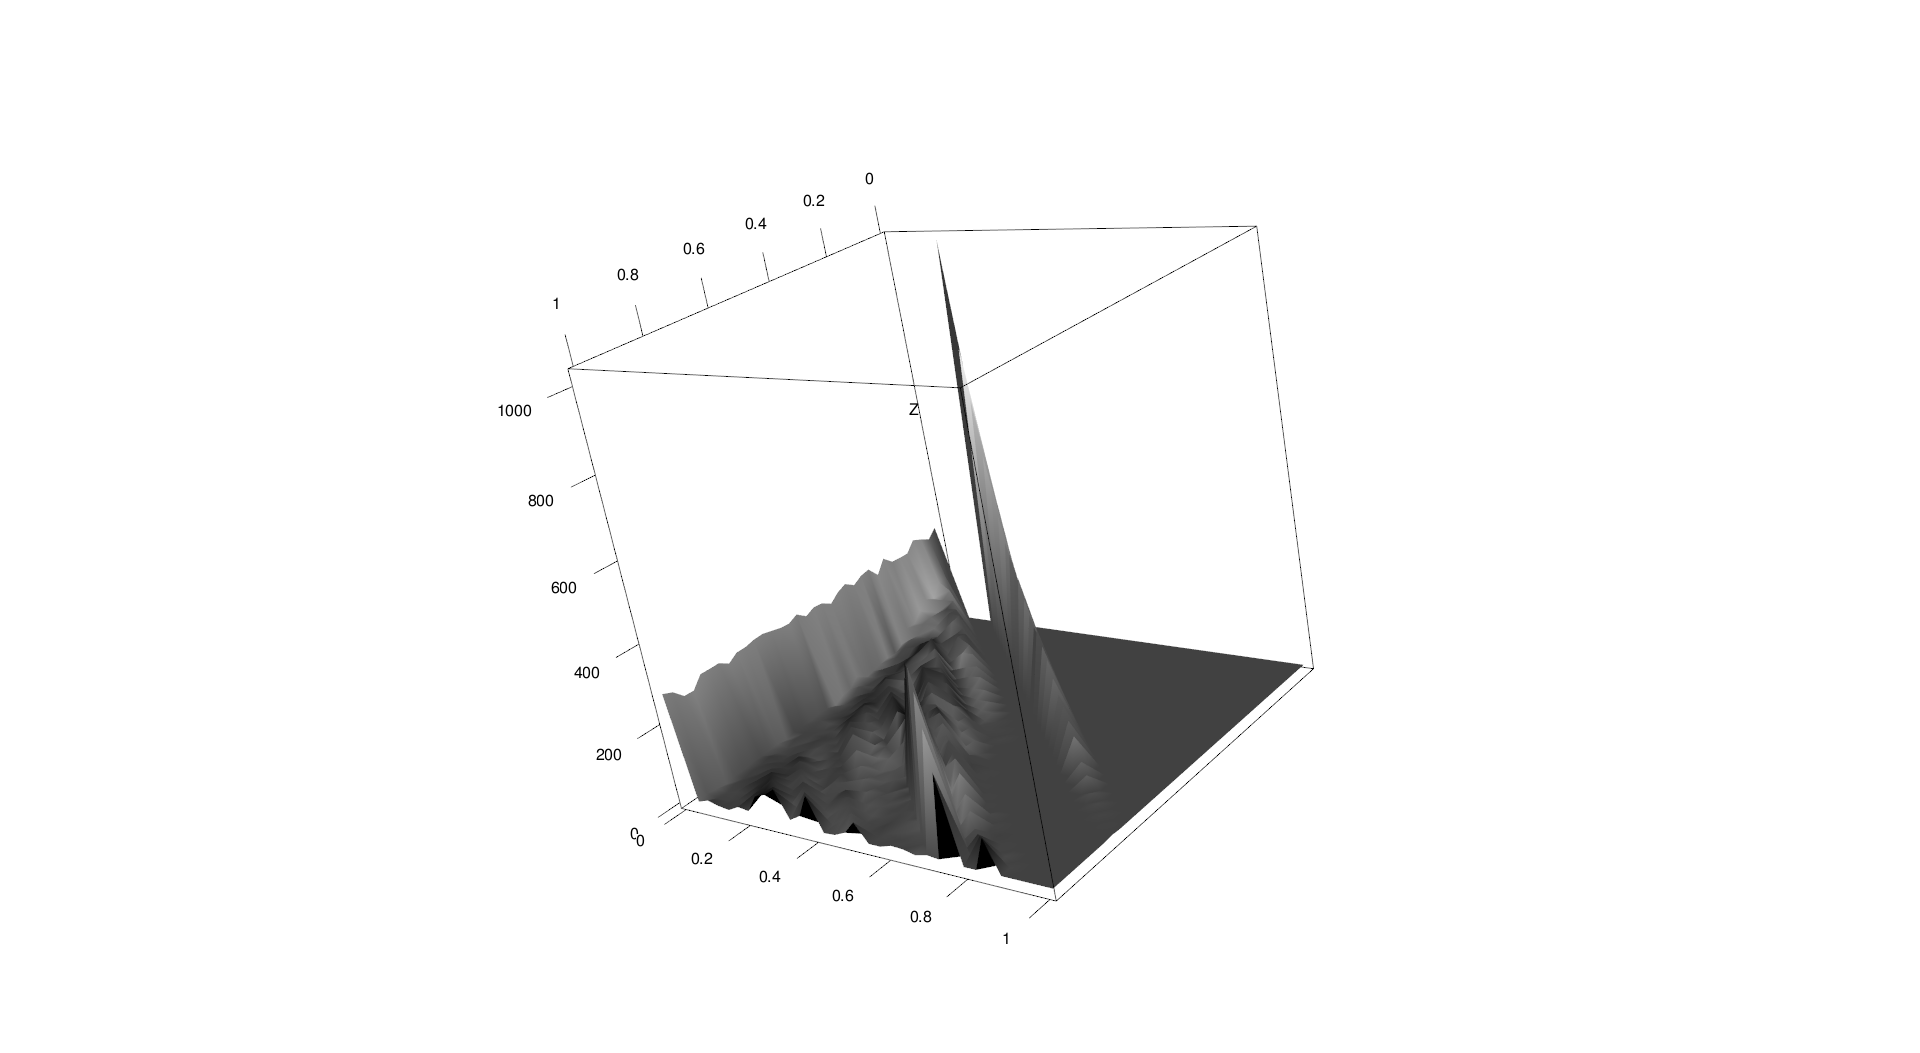
\includegraphics[width=0.5\textwidth]{memory-size.png}
}
~
\subfloat[Fitness distribution]{
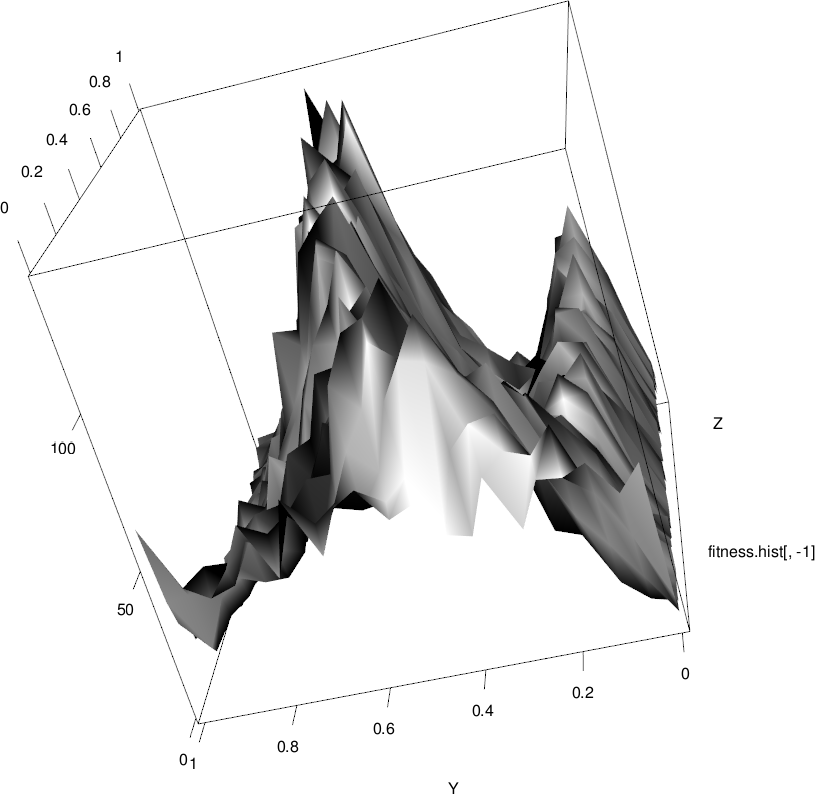
\includegraphics[width=0.5\textwidth]{fitness-distribution.png}
}
\caption{(Left) 3D plot of the distribution of memory sizes for a single
  execution of the Wilcoxon-test based partial order. Initially, all
  individuals (1024) started with 6 evaluations, which accounts for
  the peak. (Right)
  3d plot of the distribution of fitness values along time for the WPO
  method on the Trap function. \label{fig:initial}}
\end{figure}
Initial tests were made with these two types of algorithms and the
Trap function \cite{wilcoxon:ga}, showing good results for the second
type of method and both of them being better, on that problem, that
the implicit average method that uses a single noisy evaluation. The
only aspect in which this method is better is in speed and memory
footprint. Since it does not need to perform averages or make
additional fitness measures every generation, it is twice as fast as
the next method, the one that uses explicit average fitness. An
exploration of memory sizes (shown in Figure \ref{fig:initial}, left; a rotating version of the graph is published in
  \url{http://jj.github.io/Algorithm-Evolutionary/graphs/memory/}) for a
typical run) showed that there is an uneven distribution of memory
sizes and thus ages but, in general, there is no single memory size
overcoming all the population. Besides, distribution of fitness, shown
for a typical run in Figure \ref{fig:initial} (right, also published at
  \url{http://jj.github.io/Algorithm-Evolutionary/graphs/fitness-histo/}) shows a
distribution with most values concentrated along the middle (that is,
fitness equal to 10 or individuals that cannot be compared with any
other, together with a few with the highest fitness and many with the
lowest fitness. Besides showing that using the partial order is a
valid strategy, it also shows that a too greedy selection method would
eliminate many individuals that might, in fact, have a high fitness if
only given the chance to be evaluated for another generation. This
will be taken into account when assigning parameter values to the
evolutionary algorithm that will be presented next.

All these initial tests have been programmed using {\tt
  Algorithm::Evoluitionary} (in Perl) \cite{ae09} and code and data
are available under an open source licence from the library
repository at GitHub
\url{https://github.com/JJ/Algorithm-Evolutionary/}. However, it was
clear from these tests that the type of problems in which every method
works the best needs to be characterized, so we will drill further
into this with another set of experiments that will be presented
next. 

\section{Results}
\label{sec:res}
%
\begin{table}[!h]
\begin{center}
\caption{Common evolutionary algorithm parameters}
\label{fig:ga_params}
\begin{tabular}{lc}%{p{3cm}p{7cm}}
\hline\noalign{\smallskip}
\noalign{\smallskip}
Parameter & Value \\
\hline
\noalign{\smallskip}
Chromosome length & 40 (Trap) 60 (MMDP)\\
Population size & 1024.\\
Selection & 2 tournament selection \\
Replacement rate & 50\% \\
Mutation rate & 20\% \\
Crossover rate &  80\% \\
Max evaluations & 200K (Trap) 1 Million(MMDP) \\
Stopping criterion & Non-noisy best found ot max evaluations reached \\
\hline
\end{tabular}
\end{center}
\end{table}
%
ETA and WPO have been tested using two well-known benchmarks, the Trap
function and the MMDP problem. Only these two functions were chosen
because they have a different fitness landscape, are usually difficult
for an evolutionary algorithm and have been extensively used for
testing other kind of operators and algorithms. Besides, they are part
of the {\tt Algorithm::Evolutionary} standard set of fitness
functions. Several methods were tested: a baseline algorithm without
noise, that gave us an idea on the time and number of evaluations
needed to find the solution, a 0-memory (implicit average) method that
uses noisy fitness without making any special arrangement, ETA and
WPO. Evolutionary algorithm parameters (listed in Table \ref{fig:ga_params})  and code for all tests were the same (except in one
particular case. We have also used an additive noise centered in one
and different $\sigma$, which are independent of the fitness values
range. 

\begin{figure}[htb]
\centering
\subfloat[Memory size]{
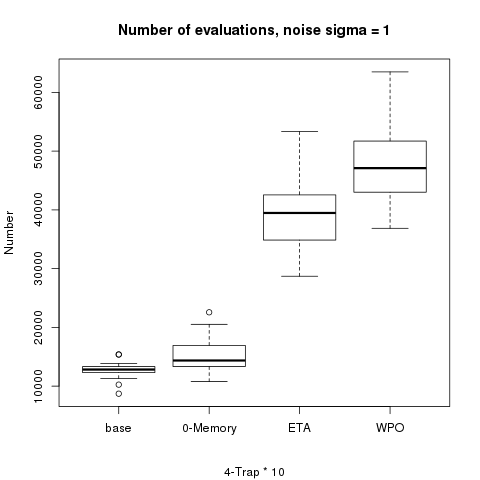
\includegraphics[width=0.5\textwidth]{trap-evals-all.png}
}
~
\subfloat[Fitness distribution]{
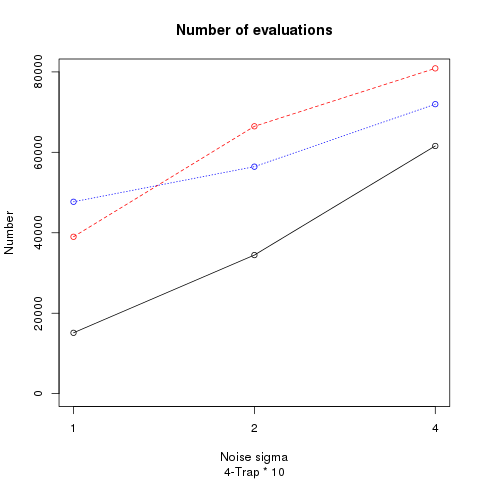
\includegraphics[width=0.5\textwidth]{trap-noisy-evals.png}
}
\caption{(Left) Comparison of number of evaluations for the 4-Trap x
  10 function and the rest of the algorithms with a noise $\sigma$
  equal to 1. (Right). Plot of average number of evaluations for
  different methods: 0 memory (black, solid), ETA (red, dashed), WPO
  (blue, dot-dashed). \label{fig:trap:evals}}
\end{figure}
%
All tests use the {\tt Algorithm::Evolutionary} library and scripts
are published, as above, in the GitHub repository, together with raw
and processed results. The evolutionary algorithm code used in all
cases is exactly the same except for WPO, which, since it needs the
whole population to evaluate fitness, needed a special reproduction
and replacement library. This also means that the replacement method
is not exactly the same: while WPO replaces every generation 50\% of
the individuals, the rest evaluate new individuals before replacement
and eliminate the worst 512 (50\% of the original
population). Replacement is, thus, less greedy in the WPO case, but
we do not think this will be a big influence on result (although it
might account for the bigger number of evaluations obtained in some
cases), besides, it just needed a small modification of code and was
thus preferred for that reason. All values shown are the result of 30
independent runs.

The results for different noise levels are shown in Figure
\ref{fig:trap:evals}. The boxplot on the left hand side compares the
number of evaluations for the baseline method and the three methods
with  $\sigma=1$. The implicit average method (labeled as 0-memory) is
only slightly worse than the baseline value of around 12K evaluations,
with the ETA and WPO method yielding very similar values which are
actually worse than the 0-memory method. However, the scenario on the
left, which shows how the number of evaluations scales with the noise
level, is somewhat different. While the 0-memory method still has the
least number of evaluations {\em for successful runs}, the success
rate degrades very fast, with roughly the same and slightly less than
100\% for $\sigma=2$ but falling down to 63\% for 0-memory and around
80\% for ETA and WPO (86\% and 80\%). That is, best success rate is
shown by the ETA method, but the best number of evaluatiosn for
roughly the same method is achieved by WPO. 

These results also show that performance degrades quickly with problem
difficulty and the degree of noise, that is why we discarded the
0-memory method due to its high degree of failure with noise = 10\%
max fitness and evaluated ETA and WPO over another problem, MMDP with
similar absolute $\sigma$, with the difference that, in this case,
$\sigma=2$ would be 20\% of the max value.

\begin{figure}[!h]
\centering
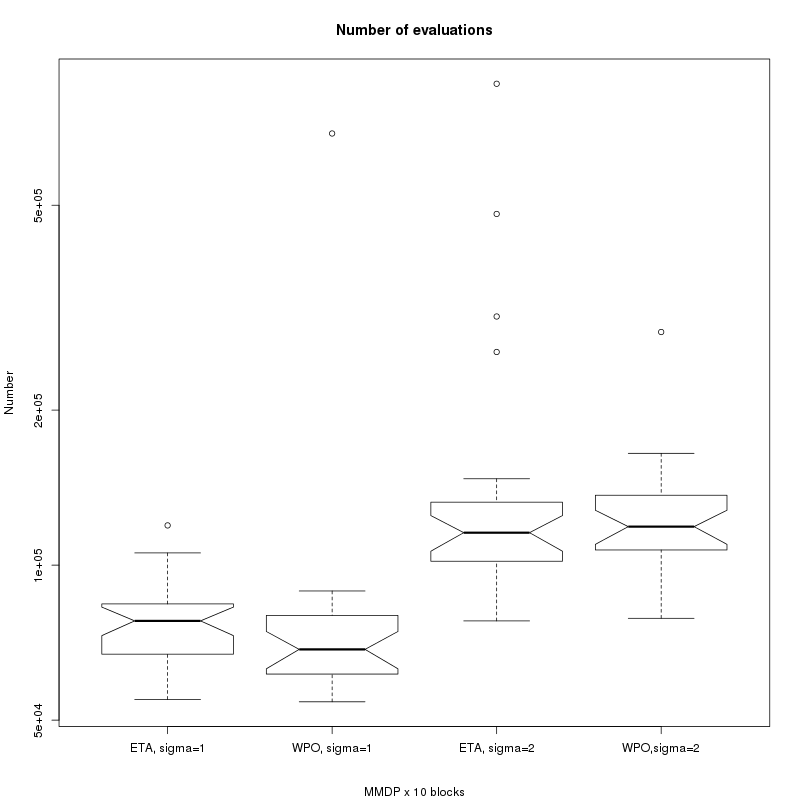
\includegraphics[width=0.7\textwidth]{evals-mmdp.png}
\caption{Number of evaluations for successful runs ETA and WPO needed for solving the MMDP
  problem with 6 blocks and different noise levels, $\sigma=1,2$. \label{fig:mmdp:evals}}
\end{figure}
%
The evolutionary algorithm for MMDP used exactly the same parameters
as for the Trap function above, except the max number of evaluations
was boosted to one million. Initial tests with the 0-memory method
yielded a very low degree of success, which left only the two methods
analyzed in this paper. Success level was in all cases around 90\%,
not different in any case, but the number of evaluations is shown in
Figure \ref{fig:mmdp:evals}. In fact, WPO and ETA have a very similar
number of evaluations. It is statistically indistinguishable for
$\sigma=2$, and different only at the 10\% level (p-value = 0.09668)
for $\sigma=1$, however, if we take time needed to reach solutions
into account, ETA is much faster since it does not apply 10*1024
statistical tests every generation. However, WPO is more robust, with
a lower standard deviation, in general, at least for high noise
levels. 

At any rate, both methods obtain a good result with a much higher
success rate than the implicit fitness method. Besides, it
incorporates explicit fitness evaluation naturally into the population
{\em resampling} only surviving individuals. This accounts for a
predictable behavior of the algorithm, since the number of evaluations
per generation is exactly the population size, which is important for
optimization processes with a limited budget. 

\section{Conclusions}



\section{Acknowledgments}

{\small This work has been supported in part by project ANYSELF
(TIN2011-28627-C04-02 and -01).
The authors would like to thank the FEDER of European Union for
financial support via project "Sistema de Informaci�n y Predicci�n de
bajo coste y aut�nomo para conocer el Estado de las Carreteras en
tiempo real mediante dispositivos distribuidos" (SIPEsCa) of the
"Programa Operativo FEDER de Andaluc�a 2007-2013". We also thank all
Agency of Public Works of Andalusia Regional Government staff and
researchers for their dedication and professionalism.}

\begin{figure}
\begin{center}

\includegraphics[width=4cm]{logos_SIPESCA_2.jpg}
\end{center}
\end{figure}

\bibliographystyle{splncs03}
\bibliography{geneura,wilcoxon}  % sigproc.bib is the name of the Bibliography in this case

\end{document}
